\documentclass[11pt,a4paper]{article}
\usepackage[utf8]{inputenc}
\usepackage[T1]{fontenc}
\usepackage{geometry}
\usepackage{graphicx}
\usepackage{fancyhdr}
\usepackage{longtable}
\usepackage{booktabs}
\usepackage{xcolor}
\usepackage{hyperref}
\usepackage{lastpage}
\usepackage{tikz}
\usetikzlibrary{shapes,arrows,positioning}

\geometry{margin=1in}

\definecolor{nis2blue}{RGB}{0,51,153}
\definecolor{nis2gray}{RGB}{100,100,100}

\pagestyle{fancy}
\fancyhf{}
\fancyhead[L]{\textcolor{nis2blue}{\textbf{Change Management Procedure}}}
\fancyhead[R]{\includegraphics[height=0.8cm]{logo.png}}
\fancyfoot[L]{\textcolor{nis2gray}{\small \jobname}}
\fancyfoot[C]{\textcolor{nis2gray}{\small Internal Use Only}}
\fancyfoot[R]{\textcolor{nis2gray}{\small Page \thepage\ of \pageref{LastPage}}}

\renewcommand{\headrulewidth}{2pt}
\renewcommand{\footrulewidth}{1pt}

\hypersetup{
    colorlinks=true,
    linkcolor=nis2blue,
    filecolor=nis2blue,
    urlcolor=nis2blue,
}

\begin{document}

\begin{titlepage}
    \centering
    \vspace*{2cm}
    {\Huge\bfseries\textcolor{nis2blue}{Change Management Procedure}\par}
    \vspace{0.5cm}
    {\Large NIS2 Directive Compliance\par}
    \vspace{2cm}
    {\Large\textbf{Organization:} [ORGANIZATION]\par}
    \vspace{0.5cm}
    {\Large\textbf{Version:} 1.0\par}
    \vspace{0.5cm}
    {\Large\textbf{Effective Date:} \today\par}
    \vfill
    {\small NIS2 Article 21(2)(e) - Security in Acquisition, Development and Maintenance\par}
\end{titlepage}

\tableofcontents
\newpage

\section{Purpose}
This procedure establishes a standardized process for planning, approving, implementing, and reviewing changes to IT systems and infrastructure while maintaining security and minimizing risk.

\section{Scope}
Applies to all changes affecting:
\begin{itemize}
    \item Production IT systems and applications
    \item Network infrastructure
    \item Security controls
    \item Databases
    \item Cloud infrastructure
    \item Critical business services
\end{itemize}

\section{Change Categories}

\subsection{Standard Change}
\textbf{Definition:} Pre-approved, low-risk, routine changes with documented procedures

\textbf{Examples:}
\begin{itemize}
    \item Routine patch deployments (approved list)
    \item User account provisioning
    \item Standard software installations
    \item Scheduled backup configuration updates
\end{itemize}

\textbf{Approval:} Pre-authorized, no CAB review required

\subsection{Normal Change}
\textbf{Definition:} Planned changes requiring CAB review and approval

\textbf{Examples:}
\begin{itemize}
    \item Application upgrades
    \item Infrastructure modifications
    \item New system deployments
    \item Configuration changes to critical systems
\end{itemize}

\textbf{Approval:} Change Advisory Board (CAB)

\subsection{Emergency Change}
\textbf{Definition:} Urgent changes required to resolve critical issues or security threats

\textbf{Examples:}
\begin{itemize}
    \item Critical security patch deployment
    \item Service restoration after outage
    \item Zero-day vulnerability remediation
    \item Critical bug fixes
\end{itemize}

\textbf{Approval:} Emergency CAB (E-CAB) or designated authority

\section{Change Management Process}

\subsection{Process Overview}

\begin{center}
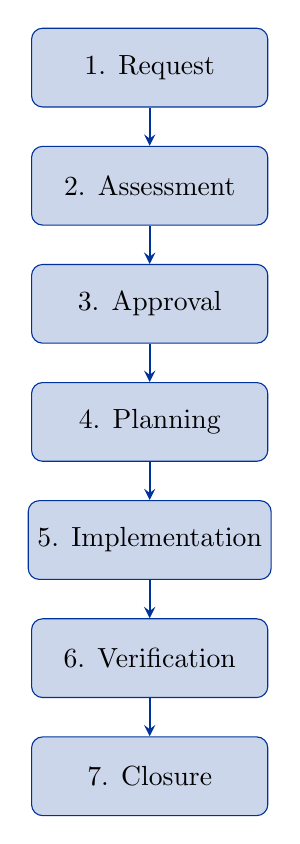
\begin{tikzpicture}[node distance=1.5cm, auto]
    \tikzstyle{box} = [rectangle, rounded corners, minimum width=3cm, minimum height=1cm, text centered, draw=nis2blue, fill=nis2blue!20]
    \tikzstyle{decision} = [diamond, minimum width=2cm, minimum height=1cm, text centered, draw=nis2blue, fill=nis2blue!20]
    \tikzstyle{arrow} = [thick,->,>=stealth,nis2blue]

    \node (request) [box] {1. Request};
    \node (assess) [box, below of=request] {2. Assessment};
    \node (approve) [box, below of=assess] {3. Approval};
    \node (plan) [box, below of=approve] {4. Planning};
    \node (implement) [box, below of=plan] {5. Implementation};
    \node (verify) [box, below of=implement] {6. Verification};
    \node (close) [box, below of=verify] {7. Closure};

    \draw [arrow] (request) -- (assess);
    \draw [arrow] (assess) -- (approve);
    \draw [arrow] (approve) -- (plan);
    \draw [arrow] (plan) -- (implement);
    \draw [arrow] (implement) -- (verify);
    \draw [arrow] (verify) -- (close);
\end{tikzpicture}
\end{center}

\subsection{Phase 1: Change Request}

\subsubsection{Initiating a Change}
All changes must be submitted via:
\begin{itemize}
    \item Change management ticketing system
    \item Change Request Form (see Appendix A)
    \item Email to: changes@[ORGANIZATION].com (for emergencies)
\end{itemize}

\subsubsection{Required Information}
\begin{itemize}
    \item Change requestor name and contact
    \item Change category (Standard/Normal/Emergency)
    \item Business justification
    \item Systems and services affected
    \item Proposed implementation date/time
    \item Estimated duration
    \item Risk assessment
    \item Rollback plan
    \item Testing plan
    \item Communication plan
\end{itemize}

\subsection{Phase 2: Assessment}

\subsubsection{Change Manager Review}
\begin{enumerate}
    \item Validate completeness of request
    \item Verify change category classification
    \item Assess impact and risk
    \item Identify dependencies
    \item Check for conflicts with other changes
    \item Determine approval path
\end{enumerate}

\subsubsection{Risk Assessment}

\begin{table}[h]
\centering
\begin{tabular}{|l|p{10cm}|}
\hline
\textbf{Risk Level} & \textbf{Criteria} \\
\hline
\textbf{High} & Affects critical systems, customer-facing services, or has potential for significant business impact \\
\hline
\textbf{Medium} & Affects important systems, requires coordination across teams, moderate business impact possible \\
\hline
\textbf{Low} & Affects non-critical systems, minimal coordination needed, limited business impact \\
\hline
\end{tabular}
\caption{Risk Assessment Criteria}
\end{table}

\subsection{Phase 3: Approval}

\subsubsection{Change Advisory Board (CAB)}

\textbf{Composition:}
\begin{itemize}
    \item Change Manager (Chair)
    \item IT Operations Manager
    \item Application Development Manager
    \item Information Security Manager
    \item Business Representative(s)
    \item Relevant Technical SMEs
\end{itemize}

\textbf{Meeting Schedule:}
\begin{itemize}
    \item Regular CAB: Weekly (Tuesdays, 10:00 AM)
    \item Emergency CAB: As needed (within 2 hours of request)
\end{itemize}

\textbf{CAB Responsibilities:}
\begin{itemize}
    \item Review change requests
    \item Assess risks and impacts
    \item Approve, reject, or defer changes
    \item Prioritize changes
    \item Authorize implementation schedule
\end{itemize}

\subsubsection{Approval Authority}

\begin{longtable}{|p{3cm}|p{3cm}|p{3cm}|p{4cm}|}
\hline
\textbf{Change Type} & \textbf{Risk Level} & \textbf{Approver} & \textbf{Timeline} \\
\hline
\endfirsthead
\hline
\textbf{Change Type} & \textbf{Risk Level} & \textbf{Approver} & \textbf{Timeline} \\
\hline
\endhead
Standard & Low & Pre-approved & Immediate \\
\hline
Normal & Low & Change Manager & 1 business day \\
\hline
Normal & Medium & CAB & Next CAB meeting \\
\hline
Normal & High & CAB + CIO & Next CAB + CIO approval \\
\hline
Emergency & Any & E-CAB or CIO/CISO & Within 2 hours \\
\hline
\caption{Approval Authority Matrix}
\end{longtable}

\subsection{Phase 4: Planning}

\subsubsection{Implementation Planning}
\begin{itemize}
    \item Detailed step-by-step procedure
    \item Resource assignment (personnel, tools, time)
    \item Communication plan
    \item Testing and validation steps
    \item Rollback procedure (mandatory)
    \item Contingency plans
\end{itemize}

\subsubsection{Change Window}

\textbf{Standard Change Windows:}
\begin{itemize}
    \item \textbf{Production Systems:} Saturdays 2:00 AM - 6:00 AM
    \item \textbf{Non-critical Systems:} Weekdays 6:00 PM - 10:00 PM
    \item \textbf{Emergency:} As required (business impact considered)
\end{itemize}

\textbf{Blackout Periods:}
\begin{itemize}
    \item Month-end close: Last 3 days of month
    \item Year-end close: December 26 - January 5
    \item Major business events: [LIST SPECIFIC DATES]
\end{itemize}

\subsubsection{Rollback Planning}
Every change must have a documented rollback plan:
\begin{itemize}
    \item Rollback triggers (when to initiate)
    \item Rollback procedure (step-by-step)
    \item Rollback time estimate
    \item Rollback authorization
    \item Data recovery procedures (if applicable)
\end{itemize}

\subsection{Phase 5: Implementation}

\subsubsection{Pre-Implementation}
\begin{enumerate}
    \item Final approval confirmation
    \item Stakeholder notification (24 hours advance)
    \item Backup verification
    \item Team readiness check
    \item Communication to users (if needed)
\end{enumerate}

\subsubsection{During Implementation}
\begin{itemize}
    \item Follow documented procedure exactly
    \item Document all actions taken
    \item Report progress at defined checkpoints
    \item Maintain communication channel open
    \item Monitor system status continuously
    \item Be prepared to execute rollback if needed
\end{itemize}

\subsubsection{Rollback Triggers}
Initiate rollback if:
\begin{itemize}
    \item Implementation exceeds allocated time window
    \item Critical errors encountered
    \item System instability observed
    \item Security issues identified
    \item Business impact exceeds acceptable threshold
    \item Unable to complete all planned steps
\end{itemize}

\subsection{Phase 6: Verification}

\subsubsection{Post-Implementation Validation}
\begin{itemize}
    \item Functional testing (verify intended outcome achieved)
    \item Performance testing (no degradation)
    \item Security validation (controls still effective)
    \item Integration testing (dependent systems working)
    \item User acceptance (if applicable)
    \item Monitoring review (no errors or alerts)
\end{itemize}

\subsubsection{Success Criteria}
Change considered successful when:
\begin{itemize}
    \item All planned changes implemented
    \item Testing confirms expected results
    \item No new errors or issues introduced
    \item System performance meets requirements
    \item No rollback required
    \item Stakeholders confirm acceptance
\end{itemize}

\subsection{Phase 7: Closure}

\subsubsection{Documentation}
Complete and attach to change record:
\begin{itemize}
    \item Implementation results
    \item Issues encountered and resolutions
    \item Actual vs. planned timeline
    \item Configuration updates
    \item Lessons learned
    \item Final sign-off
\end{itemize}

\subsubsection{Post-Implementation Review (PIR)}
Required for:
\begin{itemize}
    \item All high-risk changes
    \item Failed changes or rollbacks
    \item Changes with significant impact
\end{itemize}

\textbf{PIR Components:}
\begin{itemize}
    \item What went well
    \item What could be improved
    \item Issues and root causes
    \item Action items for improvement
    \item Knowledge base updates
\end{itemize}

\section{Emergency Change Process}

\subsection{Emergency Change Criteria}
\begin{itemize}
    \item Critical security vulnerability requiring immediate patching
    \item Major service outage requiring urgent fix
    \item Data integrity or confidentiality threat
    \item Regulatory compliance issue
    \item Customer-impacting critical defect
\end{itemize}

\subsection{Emergency Change Procedure}

\begin{enumerate}
    \item \textbf{Initiation} (0-15 min)
    \begin{itemize}
        \item Document emergency justification
        \item Contact E-CAB members
        \item Brief summary of change and risk
    \end{itemize}

    \item \textbf{Approval} (15-30 min)
    \begin{itemize}
        \item E-CAB review (virtual meeting or email)
        \item CIO or CISO approval
        \item Document approval in ticket
    \end{itemize}

    \item \textbf{Implementation} (30 min - 4 hours)
    \begin{itemize}
        \item Execute change per documented plan
        \item Continuous communication
        \item Rollback available
    \end{itemize}

    \item \textbf{Follow-up} (within 48 hours)
    \begin{itemize}
        \item Present to full CAB (next meeting)
        \item Complete documentation
        \item Conduct PIR if needed
    \end{itemize}
\end{enumerate}

\subsection{Emergency Change Authority}

In order of preference:
\begin{enumerate}
    \item Emergency CAB (if convened)
    \item CIO or CISO jointly
    \item On-call IT Manager + Security Manager
\end{enumerate}

\section{Metrics and Reporting}

\subsection{Key Performance Indicators}

\begin{longtable}{|p{6cm}|p{3cm}|p{4cm}|}
\hline
\textbf{Metric} & \textbf{Target} & \textbf{Frequency} \\
\hline
\endfirsthead
\hline
\textbf{Metric} & \textbf{Target} & \textbf{Frequency} \\
\hline
\endhead
Change success rate & >95\% & Monthly \\
\hline
Emergency changes & <10\% of total & Monthly \\
\hline
Rollbacks & <5\% of changes & Monthly \\
\hline
Unauthorized changes detected & 0 & Monthly \\
\hline
CAB attendance & >80\% & Monthly \\
\hline
Post-implementation review completion & 100\% & Monthly \\
\hline
\caption{Change Management KPIs}
\end{longtable}

\subsection{Monthly Change Report}
\begin{itemize}
    \item Total changes by category
    \item Success vs. failure rate
    \item Rollback statistics
    \item Changes by system/application
    \item Incident correlation (changes causing incidents)
    \item Trends and analysis
\end{itemize}

\section{Roles and Responsibilities}

\subsection{Change Manager}
\begin{itemize}
    \item Overall change process ownership
    \item CAB meeting facilitation
    \item Change request review and triage
    \item Conflict identification and resolution
    \item Metrics and reporting
    \item Process improvement
\end{itemize}

\subsection{Change Advisory Board (CAB)}
\begin{itemize}
    \item Review and approve/reject changes
    \item Risk assessment
    \item Priority setting
    \item Schedule authorization
\end{itemize}

\subsection{Change Requestor}
\begin{itemize}
    \item Submit complete change request
    \item Provide accurate information
    \item Develop implementation and rollback plans
    \item Execute approved changes
    \item Document results
\end{itemize}

\subsection{Technical Teams}
\begin{itemize}
    \item Execute approved changes
    \item Provide technical expertise
    \item Test and validate changes
    \item Support rollback if needed
\end{itemize}

\subsection{Business Stakeholders}
\begin{itemize}
    \item Define business requirements
    \item Accept business risk
    \item Participate in UAT
    \item Approve business-impacting changes
\end{itemize}

\section{Change Freeze}

\subsection{Freeze Periods}
Change freezes may be declared for:
\begin{itemize}
    \item Critical business periods
    \item Major incidents or crises
    \item System stability concerns
    \item Regulatory audits
\end{itemize}

\subsection{Freeze Exceptions}
During a freeze, only these changes permitted:
\begin{itemize}
    \item Critical security patches
    \item Emergency fixes for service outages
    \item Changes with CIO/CEO approval
\end{itemize}

\section{Compliance and Audit}

\subsection{Record Retention}
\begin{itemize}
    \item Change records: 3 years
    \item CAB meeting minutes: 3 years
    \item Post-implementation reviews: 2 years
\end{itemize}

\subsection{Audit Requirements}
\begin{itemize}
    \item Quarterly change management audit
    \item Sample testing of change records
    \item Authorization verification
    \item Procedure compliance review
    \item Unauthorized change detection
\end{itemize}

\section{Related Documents}
\begin{itemize}
    \item Cybersecurity Policy
    \item Incident Response Plan
    \item Vulnerability Management Procedure
    \item Asset Management Policy
    \item Configuration Management Database (CMDB)
\end{itemize}

\section{Appendices}

\subsection{Appendix A: Change Request Form}
[Template for change request submission]

\subsection{Appendix B: CAB Meeting Agenda Template}
[Standard agenda for CAB meetings]

\subsection{Appendix C: Post-Implementation Review Template}
[Template for conducting PIR]

\section{Approval}
\begin{table}[h]
\centering
\begin{tabular}{|l|l|l|}
\hline
\textbf{Role} & \textbf{Name} & \textbf{Date} \\
\hline
Change Manager & & \\
\hline
CIO & & \\
\hline
CISO & & \\
\hline
\end{tabular}
\end{table}

\end{document}
